\documentclass[12pt]{article}
\usepackage[utf8]{inputenc}
\usepackage{graphicx}

\begin{document}

\begin{center}
\textbf{Supplementary material for:}\\
\emph{Enabling high resolution hydrologic routing with machine learning assisted waterbody classification}
\end{center}

\begin{figure}[h!]
    \begin{center}
          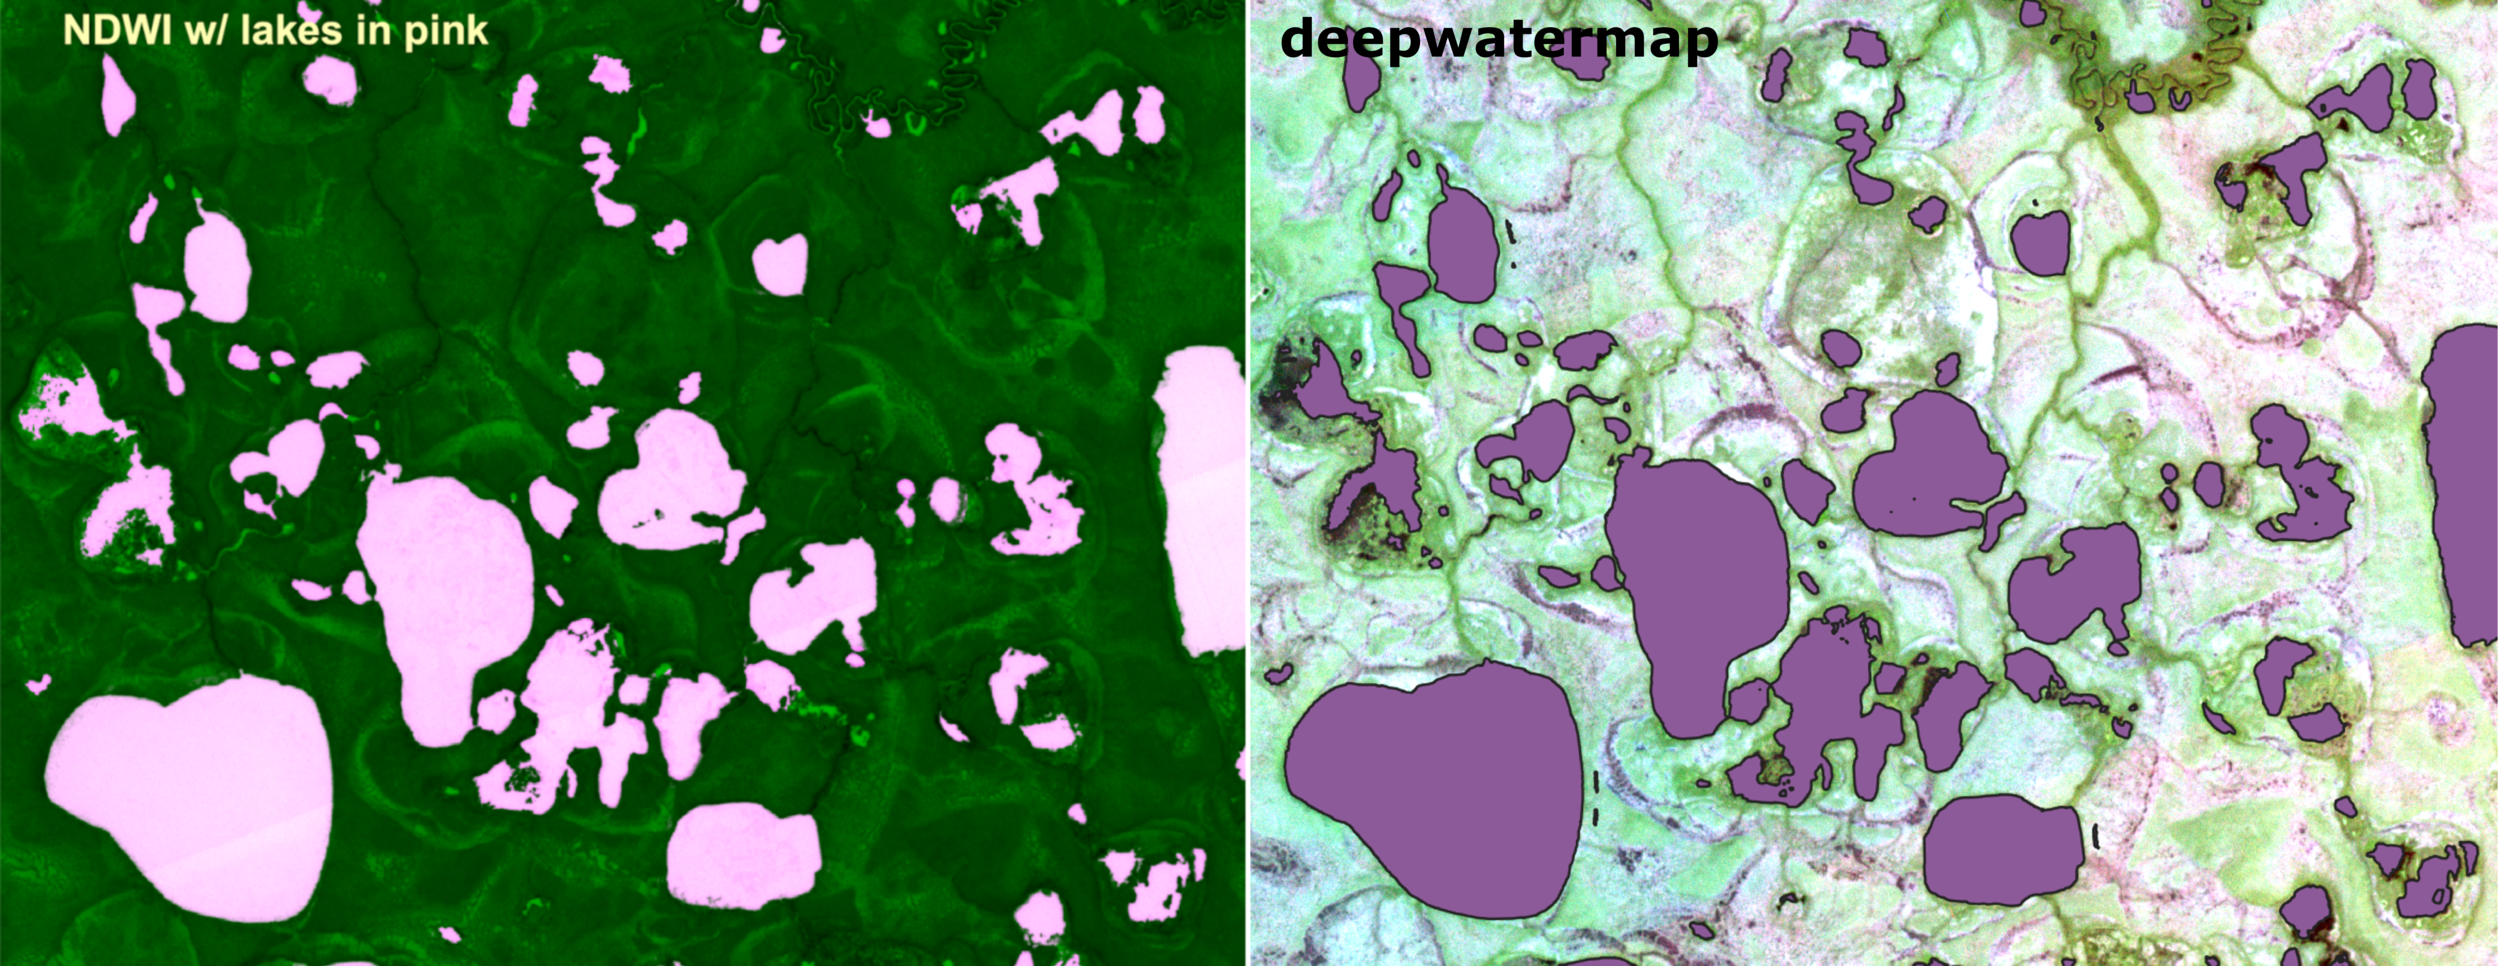
\includegraphics[width=0.7\textwidth,keepaspectratio]{../figures/deepwatermap_vs_ndwi}
          \caption{Demonstration of the similarities between candidate waterbody polygons identified with a simple normalized difference water index (NDWI) algorithm (left) and the neural-network based DeepWaterMap tool (right).}
    \end{center}    
    % Overlaying the two would be the most useful (e.g. black background, white where overlap, magenta where only NDWI, cyan where only DWM) - jschwenk
\end{figure}

\clearpage


\end{document}